%------------------------------------------------------------------------
% Presentation example for students by Markus Koschi
%
% compile with LaTeX + dvips + ps2pdf or 
% compile with PdfLaTeX after removing all eps figures 

%------------------------------------------------------------------------
\documentclass[shortpres,aspectratio=43]{beamer}
%\documentclass[shortpres,aspectratio=169]{beamer}
\usetheme{CambridgeUS}
\usepackage{svg}
%Graphics and Videos
\usepackage{graphicx} %The mode "LaTeX => PDF" allows the following formats: .jpg  .png  .pdf  .mps
\graphicspath{{./PresentationPictures/}} %Where the figures folder is located
\usepackage{media9}
\addmediapath{./Movies/}

\setbeamertemplate{footline}
{
  \leavevmode%
  \hbox{%
  \begin{beamercolorbox}[wd=.333333\paperwidth,ht=2.25ex,dp=1ex,left]{author in head/foot}%
  \hspace*{4ex}\usebeamerfont{author in head/foot} Practical Course
  \end{beamercolorbox}%
  \begin{beamercolorbox}[wd=.333333\paperwidth,ht=2.25ex,dp=1ex,center]{title in head/foot}%
    \usebeamerfont{title in head/foot} MPFAV
  \end{beamercolorbox}%
  \begin{beamercolorbox}[wd=.333333\paperwidth,ht=2.25ex,dp=1ex,right]{date in head/foot}%
    \usebeamerfont{date in head/foot}\insertshortdate{}\hspace*{2em}
    \insertframenumber{} / \inserttotalframenumber\hspace*{2ex}
  \end{beamercolorbox}}%
  \vskip0pt%
}\part{title}
\beamertemplatenavigationsymbolsempty

%color specification-----------------------------------------------------
\definecolor{TUMblue}{RGB}{27, 94, 170}%{rgb}{0.00, 0.40, 0.74}
\definecolor{TUMgray}{rgb}{0.85, 0.85, 0.86}
\definecolor{TUMpantone285C}{rgb}{0.00, 0.45, 0.81}
\definecolor{TUMpantone300C}{RGB}{27, 94, 170} %uncorrected TUMpantone300C
\definecolor{lightblue}{RGB}{213,227,241}%{rgb}{0.7529,0.8118,0.9333}

\setbeamercolor{block title}{fg=white, bg=TUMblue}
\setbeamercolor{block body}{bg=lightblue}
\setbeamertemplate{blocks}[rounded][shadow=true]

%------------------------------------------------------------------------
\setbeamercolor{frametitle}{bg=TUMblue, fg=white}
\setbeamercolor{palette primary}{bg=TUMblue, fg=white}%{fg=TUMblue,bg=TUMgray}
\setbeamercolor{palette secondary}{use=palette primary,bg=TUMblue, fg=white}
\setbeamercolor{palette tertiary}{use=palette primary,fg=white, bg=TUMblue}
\setbeamercolor{palette quaternary}{use=palette primary,fg=white, bg=TUMblue}

\setbeamercolor{title}{bg=TUMblue,fg=white}
\setbeamercolor{item projected}{use=item,fg=black,bg = lightblue}
\setbeamercolor{block title}{fg=black, bg=lightblue}
\setbeamercolor{block body}{bg=white}
\setbeamertemplate{blocks}[rounded][shadow=true]

%------------------------------------------------------------------------
\setbeamertemplate{bibliography item}{\insertbiblabel}
\setbeamercolor{bibliography item}{parent=palette primary}
\setbeamercolor{bibliography entry author}{fg=TUMblue}

%------------------------------------------------------------------------
\usepackage{subfigure}
\usepackage{textpos} % for figure (logo) on slides
\usepackage{psfrag} % for \psfrag in figures
%\usepackage{algorithm,algpseudocode} % for algorithm environment
%\usepackage{booktabs} % for rulers in tables
\usepackage{units} % for units to values
%\usepackage{hyperref}
%\usepackage{graphicx}

%-----------------------------------------------------------------------
\newcommand{\at}{\fontfamily{ptm}\selectfont @}
\newcommand{\ra}[1]{\renewcommand{\arraystretch}{#1}} %to change the row spacing in tables

\newcommand\blfootnote[1]{%
  \begingroup
  \renewcommand\thefootnote{}\footnote{#1}%
  \addtocounter{footnote}{-1}%
  \endgroup
}

%-----------------------------------------------------------------------
\title[Title]{Scene-aware and Social-aware Motion
Prediction for Autonomous Driving}

\author[Name]{Alfred Nguyen, Baris Sözüdogru}
\institute[TU M\"unchen]{Technical University of Munich}

\date{January~06,~2024}


% Print this at the beginning of each section
\AtBeginSection[]
{
  \begin{frame}
    \frametitle{Agenda}
    \tableofcontents[currentsection]
  \end{frame}
}




%---------------------------------------------------------------------
\begin{document}

%% TUM logo
\addtobeamertemplate{frametitle}{}{%
\begin{textblock*}{\textwidth}(.91\textwidth,-0.925cm) % for aspectratio=43

\includegraphics[height=0.65cm]{./figures/TUM_Logo_weiss_e.eps} % for aspectratio=43
%\begin{textblock*}{\textwidth}(.92\textwidth,-0.93cm) % for aspectratio=169
%
\includegraphics[height=0.7cm]{./figures/TUM_Logo_weiss_e.eps} % for aspectratio=169
\end{textblock*}}


\begin{frame}[plain]
    \titlepage
\end{frame}

\begin{frame}
  \frametitle{Agenda}
  \tableofcontents
\end{frame}


%
\section{Motivation}





\section{Method Description}

\subsection{The Dataset Collection}
\begin{frame}
  \frametitle{Dataset Collection}
  \begin{figure}[!t]
    \centering
    \begin{minipage}[h]{0.32\linewidth}
        \begin{block}{exiD}
            \centering
            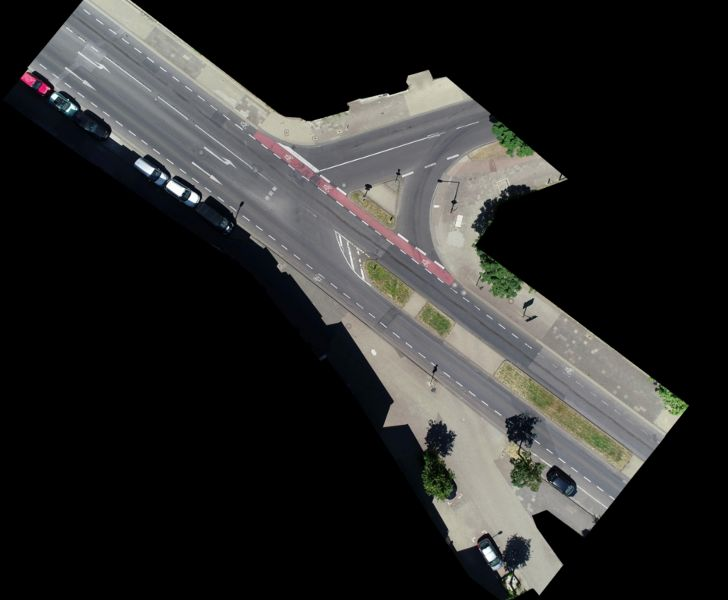
\includegraphics[width=\textwidth]{figures/pictures_first_part/inD.jpeg}
        \end{block}
    \end{minipage}
    \begin{minipage}[h]{0.32\linewidth}
        \begin{block}{rounD}
            \centering
            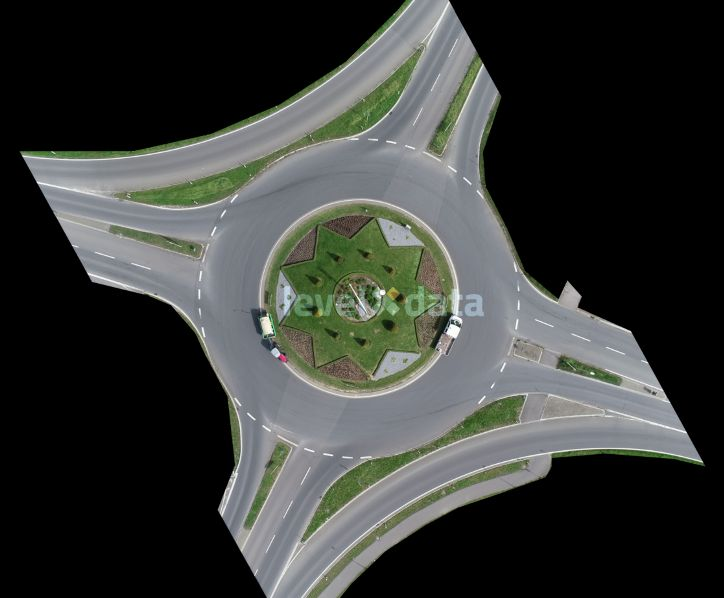
\includegraphics[width=\textwidth]{figures/pictures_first_part/rounD.jpeg}
        \end{block}
    \end{minipage}
    \begin{minipage}[h]{0.32\linewidth}
        \begin{block}{inD}
            \centering
            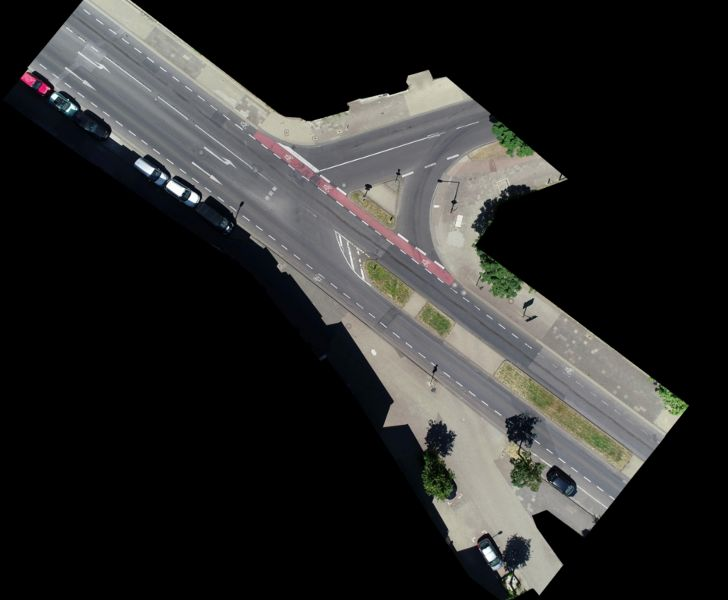
\includegraphics[width=\textwidth]{figures/pictures_first_part/inD.jpeg}
        \end{block}
    \end{minipage}
  \end{figure}
\end{frame}

\begin{frame}
  \frametitle{Method Description - Overview}
    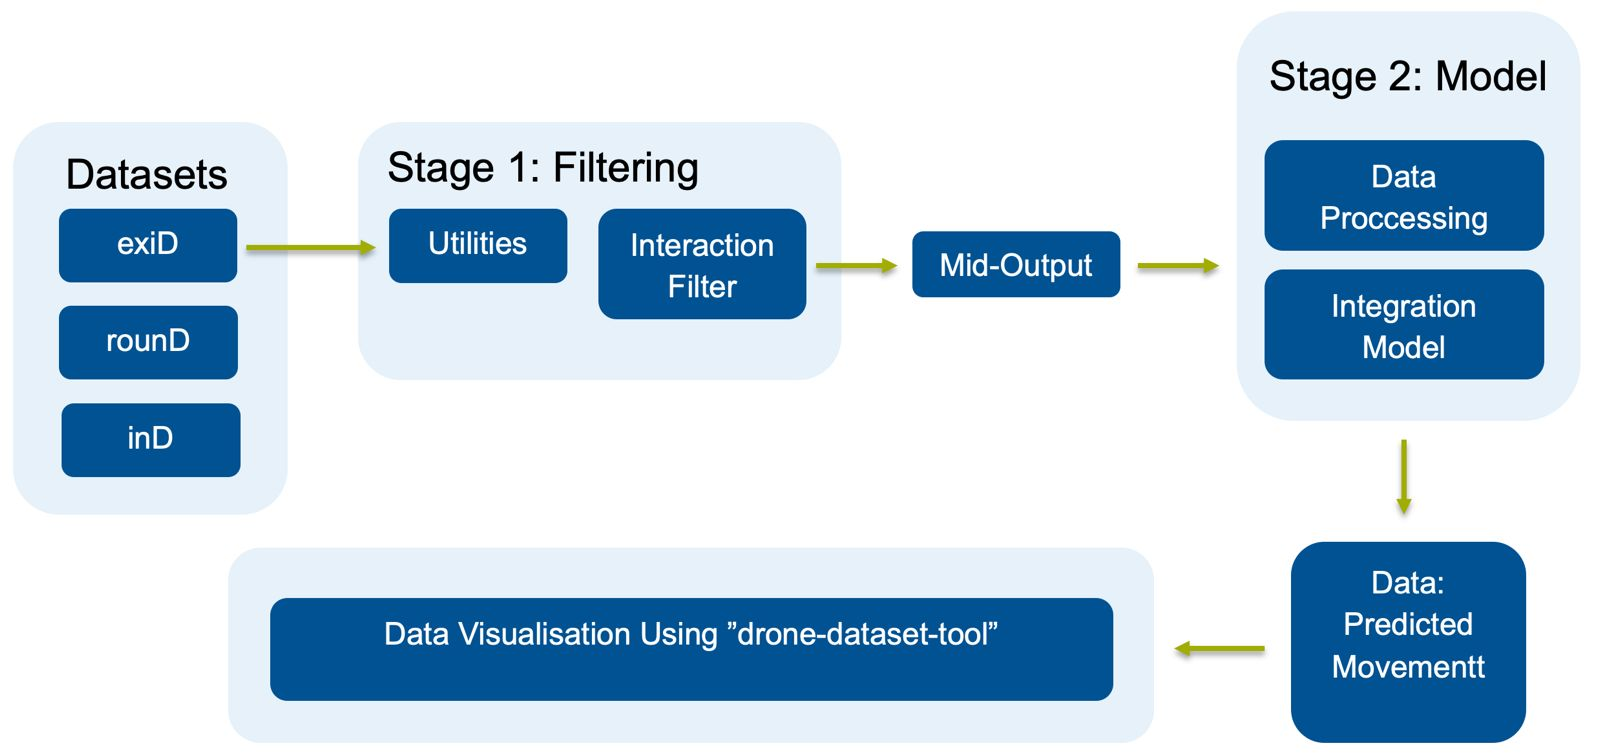
\includegraphics[width=\textwidth]{figures/pictures_first_part/method_overview.jpeg}
\end{frame}

\subsection{Stage 1 - Filtering process}

\begin{frame}
  \frametitle{Method Description - Stage 1}
    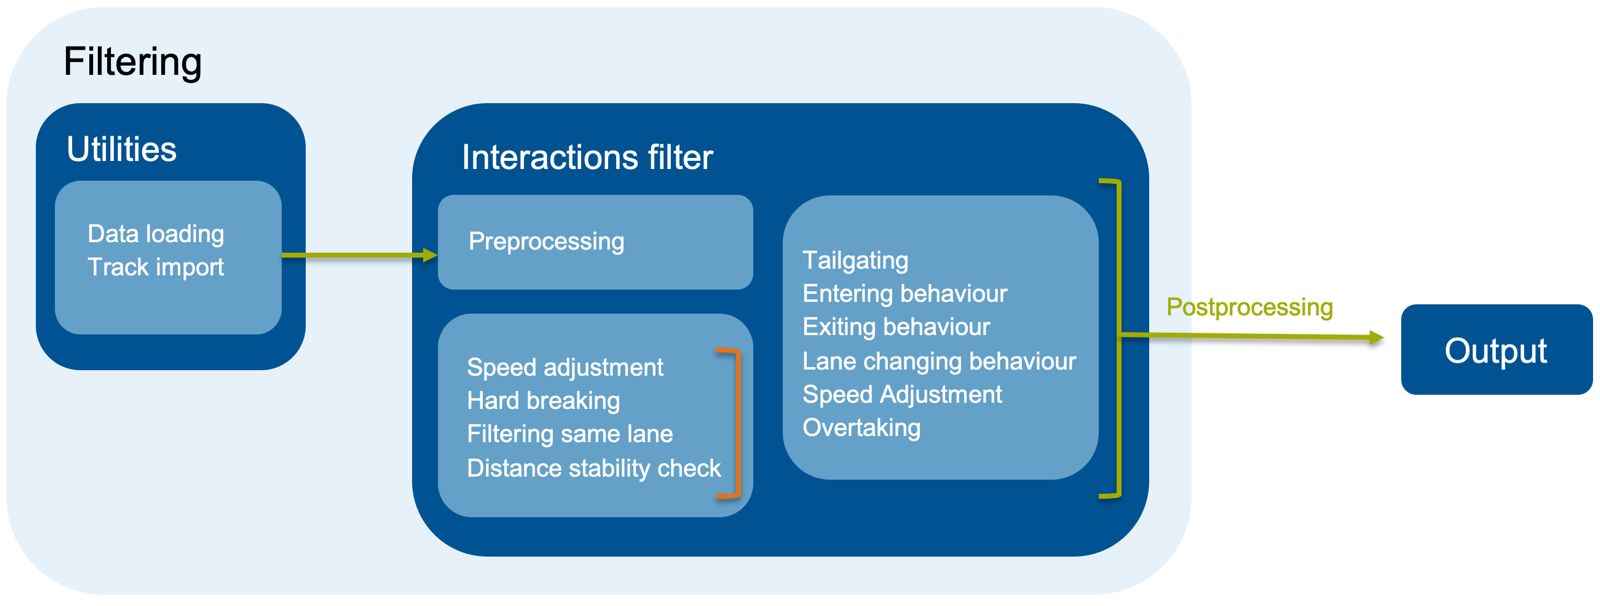
\includegraphics[width=\textwidth]{figures/pictures_first_part/filtering_overview.jpeg}
\end{frame}


\begin{frame}

  \frametitle{Method Description - Stage 1}
  \begin{figure}

    \centering
    \begin{minipage}[b]{0.49\linewidth}
        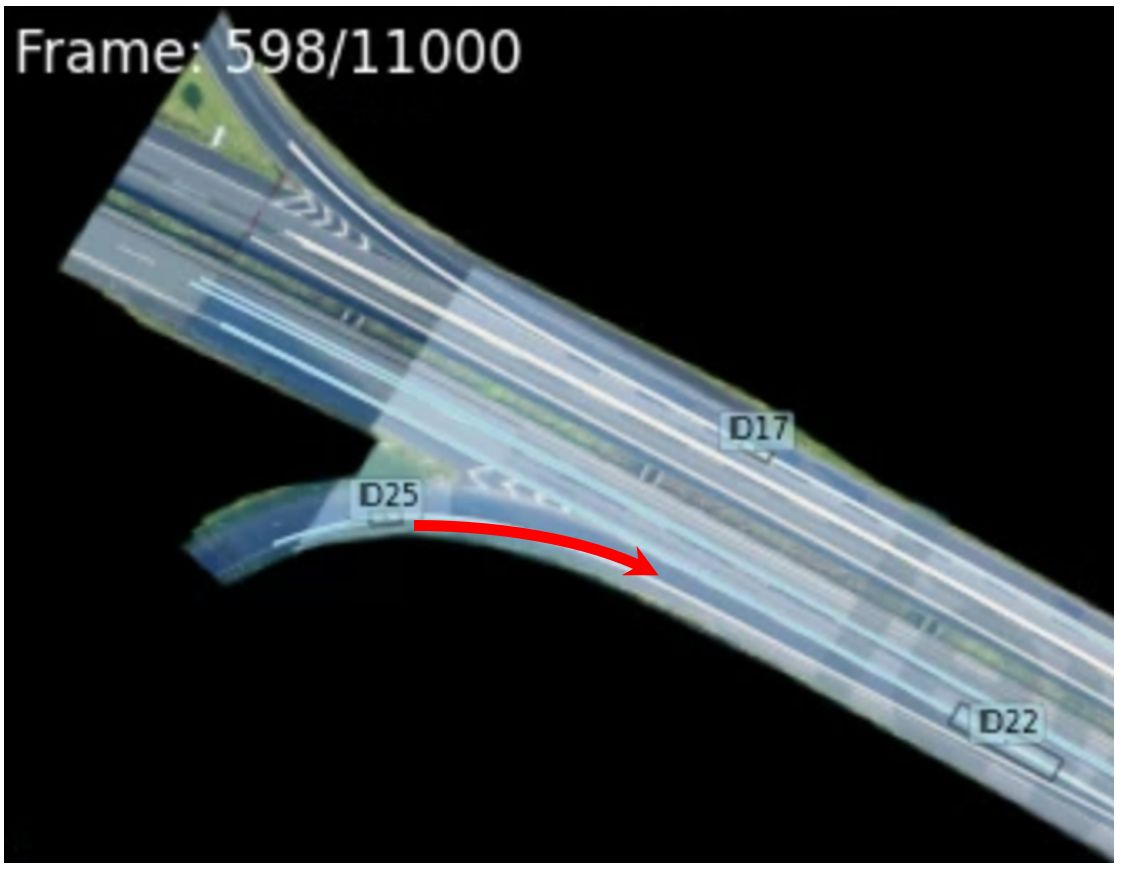
\includegraphics[width=\textwidth]{figures/pictures_first_part/street_with_arrow.jpeg}

        \centering \footnotesize Merging Lane Entering Scenario
    \end{minipage}
    \begin{minipage}[b]{0.49\linewidth}

        \centering
        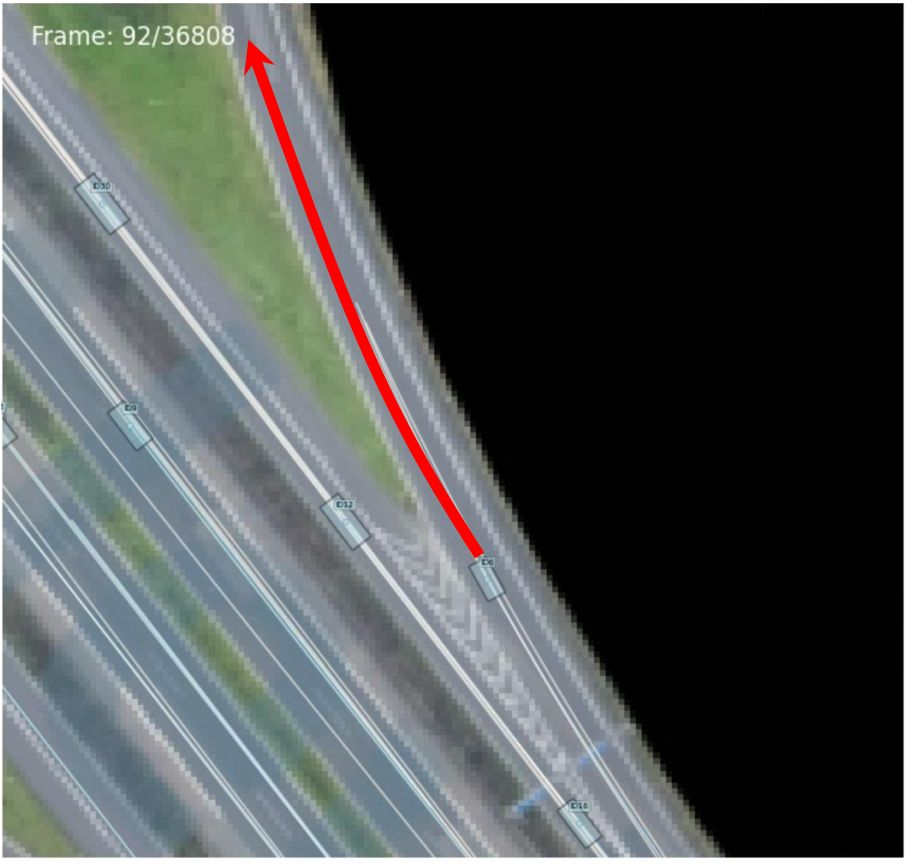
\includegraphics[width=0.82\textwidth]{figures/pictures_first_part/street_with_arrow_2.jpeg}

        \centering \footnotesize Merging Lane Exiting Scenario
    \end{minipage}
  \end{figure}
\end{frame}

\begin{frame}
  \frametitle{Method Description - Stage 1}

  \begin{figure}

    \begin{minipage}[b]{0.64\linewidth}
      \textbf{Filtering Stage: Identifying Vehicle \\ Behaviors}
      \begin{itemize}
          \item Preprocessing
          \item Behavior Detection
              \begin{itemize}
                  \item Entering/Exiting Behavior
              \end{itemize}
          \item Interaction Analysis
          \item Lane Change Detection
          \item Thresholds and Conditions
          \item Data Grouping and Sorting
      \end{itemize}
    \end{minipage}
    \begin{minipage}[b]{0.35\linewidth}

        \centering
        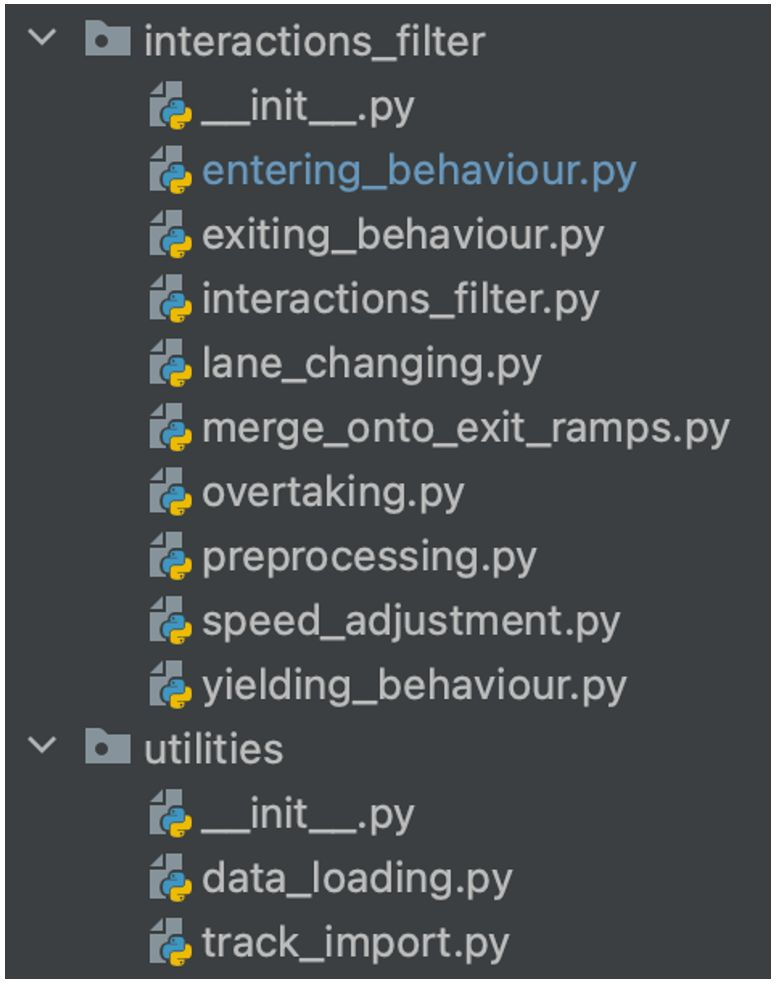
\includegraphics[width=1\textwidth]{figures/pictures_first_part/python_code_filter.jpeg}
    \end{minipage}
  \end{figure}
\end{frame}

\subsection{Stage 2 - Integration Model}

\begin{frame}
  \frametitle{Method Description - Stage 2}
    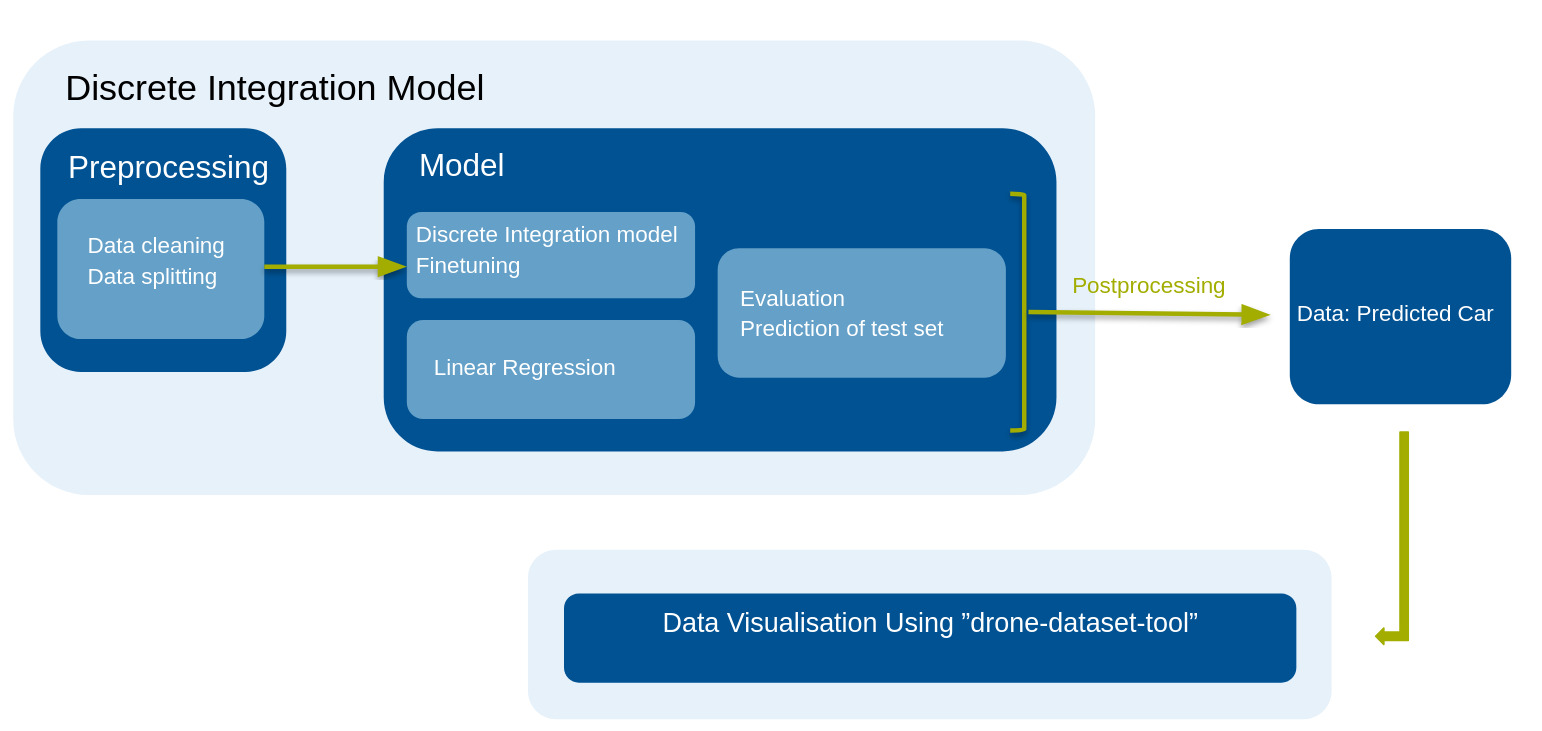
\includegraphics[width=\textwidth]{figures/pictures_second_part/integration_overview.jpeg}
\end{frame}



\begin{frame}
  \frametitle{Method Description - Stage 2}
    Distance and Velocity Equations:
\onslide<2, 3, 4>{
    \begin{align*}
    s(k+1) &= s(k) + dt \cdot v(k)+ \textcolor{red}{c_1} a(k) + \textcolor{red}{c_2} a(k-1) \\
    v(k+1) &= v(k) +                \textcolor{red}{c_3} a(k) +                \textcolor{red}{c_4} a(k-1)
    \end{align*}

    \hfil
}
\onslide<3, 4>{

    Acceleration Equations:
    \begin{align*}
    a(k) &= - \overline{\textcolor{red}{c_1}} a(k-1)  + \overline{\textcolor{red}{c_2}} \bigl( s(k+1) - s(k) - dt \cdot  v(k)\bigr)\\
    a(k) &= - \overline{\textcolor{red}{c_3}} a(k-1)  + \overline{\textcolor{red}{c_4}} \bigl( v(k+1) - v(k) \bigr) 
    \end{align*}

}


  \onslide<4->{
  Note: 
    \begin{itemize}
          \item The acceleration resulting from both formulas should be equal
          \item Model can be solved using linear regression.
      \end{itemize}
  }


\end{frame}




\section{Results}

\subsection{Filtering Process}

\begin{frame}
  \frametitle{Scenario filtering}
  \center Video demo of the scenarios
\end{frame}


\subsection{Integration Method}

\begin{frame}
  \frametitle{Results: Comparison to the old acceleration model}

  \begin{figure}

    \centering
    \begin{minipage}[b]{0.49\linewidth}

  \onslide<1, 2>{
        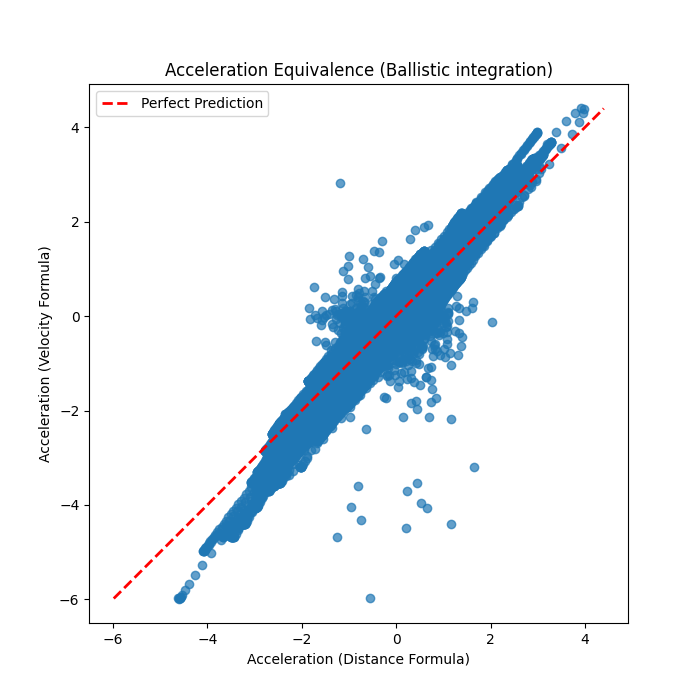
\includegraphics[width=\textwidth]{figures/graphs/Acceleration Equivalence (Ballistic integration).png}

        \centering \footnotesize MSE: 3.0786e+02
  }
    \end{minipage}
    \begin{minipage}[b]{0.49\linewidth}

  \onslide<2>{
        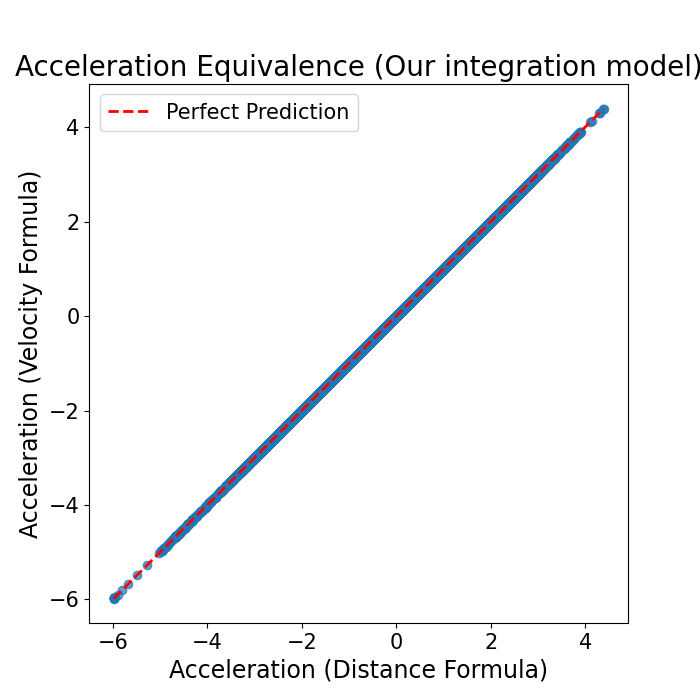
\includegraphics[width=\textwidth]{figures/graphs/Acceleration Equivalence (Our integration model).png}
        \centering \footnotesize MSE: 1.9220e-09
  }
    \end{minipage}
  \end{figure}
\end{frame}






\begin{frame}
  \frametitle{Results: Integration Method}
    Rearranging the formula to the distance and velocity gives us these results:
    \center \textit{Video demo of predicted car}
\end{frame}


%
\section{Future Work}
\begin{frame}
  \frametitle{Agenda}
  \tableofcontents[currentsection, currentsubsection]
\end{frame}
\begin{frame}
    \frametitle{Future Work}

    Scenario Filtering:

    \begin{itemize}[<+->]
        \item Specify even more scenarios for a broader range of use cases.
        \item Explore other datasets 
    \end{itemize}

    \hfil

    \onslide<3,4>{
    Integration Model:
    \begin{itemize}[<+->]
        \item Finetune the integration model (adding other parameteres)
        \item Test the integration model with the neural network for performance (task for the next team)
    \end{itemize}
}

\end{frame}


%\section{Test}

\begin{frame}
\end{frame}


\begin{frame}
\end{frame}


\begin{frame}
\end{frame}


\begin{frame}
\end{frame}


\begin{frame}
\end{frame}


\begin{frame}
  \frametitle{Acceleration Modification in the Y-axis}
  \begin{figure}
    \centering
    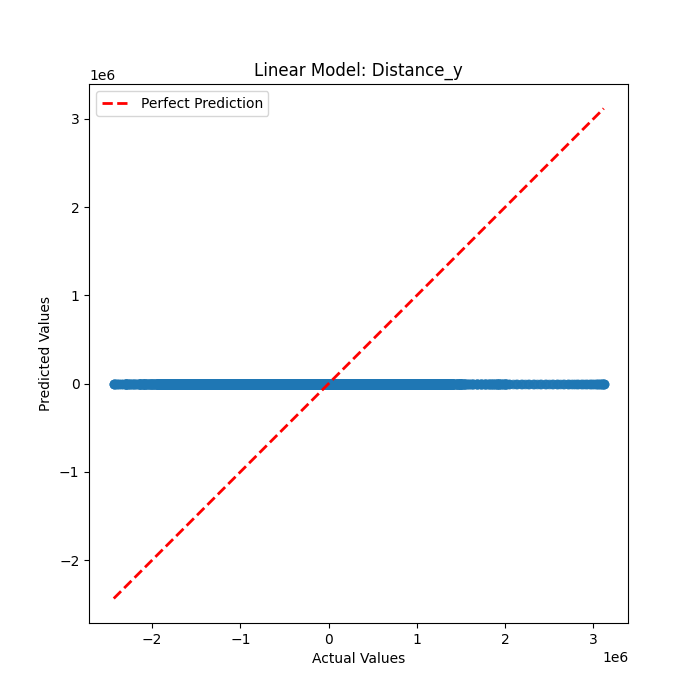
\includegraphics[width=0.5 \textwidth]{figures/acceleration_mod/acceleration_mod_dist_y.png}
  \end{figure}
\end{frame}


\begin{frame}
  \frametitle{Acceleration Modification in the Y-axis}
  \begin{figure}
    \centering
    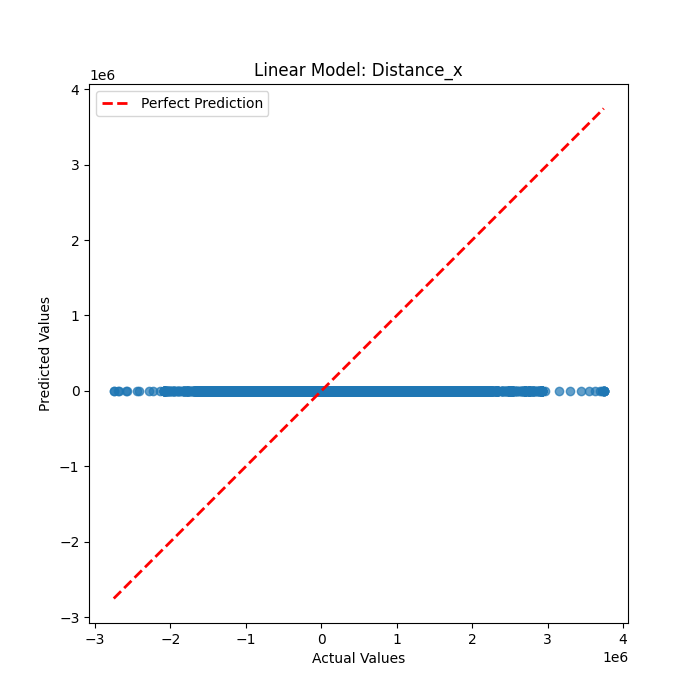
\includegraphics[width=0.5 \textwidth]{figures/acceleration_mod/acceleration_mod_dist_x.png}
  \end{figure}
\end{frame}


\begin{frame}
  \frametitle{Acceleration Modification in the Y-axis}
  \begin{figure}
    \centering
    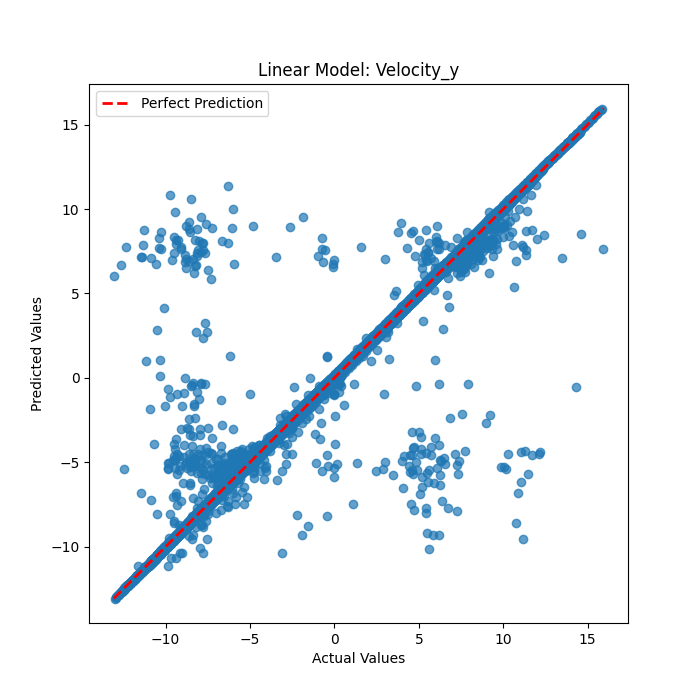
\includegraphics[width=0.5 \textwidth]{figures/acceleration_mod/acceleration_mod_vel_y.png}
  \end{figure}
\end{frame}


\begin{frame}
  \frametitle{Acceleration Modification in the Y-axis}
  \begin{figure}
    \centering
    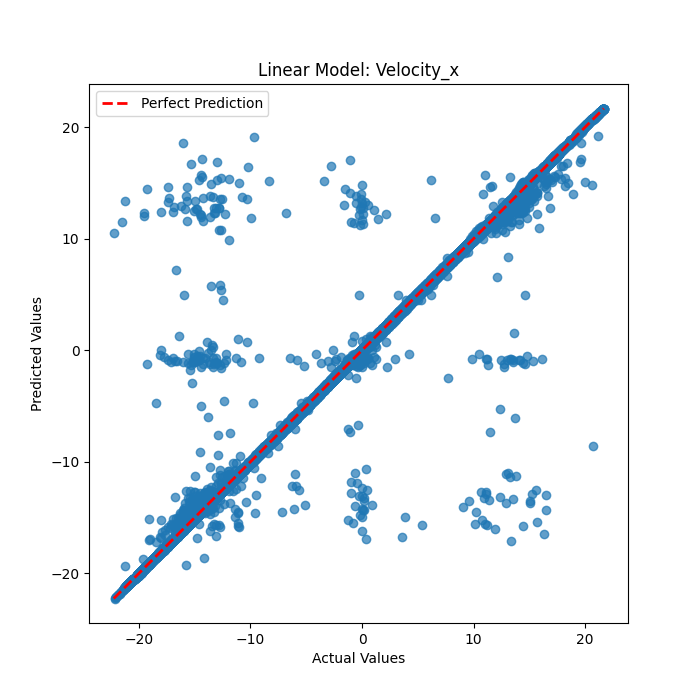
\includegraphics[width=0.5 \textwidth]{figures/acceleration_mod/acceleration_mod_vel_x.png}
  \end{figure}
\end{frame}




\begin{frame}{Motivation for Set-Based Prediction $[$1$]$}
\blfootnote{\tiny $[$1$]$ M. Althoff and S. Magdici, ``Set-based prediction of traffic participants on arbitrary road networks,'' IEEE Transactions on Intelligent Vehicles, vol. 1, no. 2, pp. 187--202, 2016.}

	\centering	
	\footnotesize
      \psfrag{o}[c][c]{obstacle}						
      \psfrag{c}[c][c]{traffic participant}
      \psfrag{e}[c][c]{ego vehicle}
      \psfrag{f}[c][c]{intended trajectory}      
      \psfrag{w}[r][c]{$t \in [t_0, t_1]$:}
      \psfrag{x}[r][c]{$t \in [t_1, t_2]$:}
      \psfrag{y}[r][c]{$t \in [t_2, t_3]$:}
      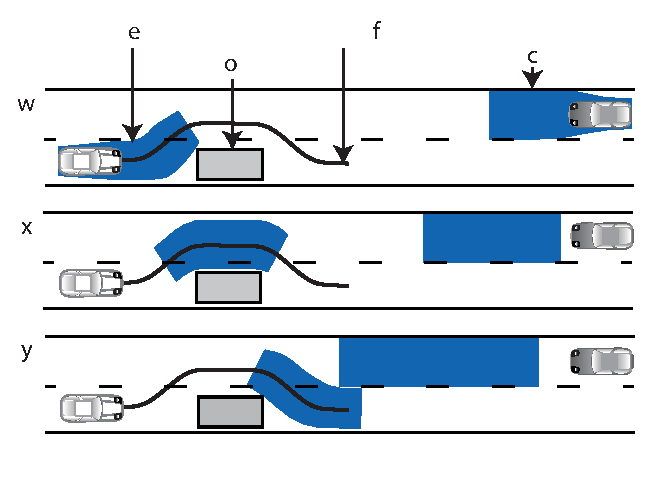
\includegraphics[width=0.8\columnwidth, height=0.74\textheight, keepaspectratio]{./figures/snapshots_blue.eps}
      %\caption{Snapshots of the predicted occupancy of the traffic participant for selected consecutive time intervals.}
\end{frame}


%\begin{frame}{Outline}
%\begin{enumerate}
%\item Item
%\vfill \item Item
%\vfill \item Item
%\vfill \item Item
%\vfill \item Item
%\end{enumerate} 
%\end{frame}



\begin{frame}{SPOT}
SPOT: A tool for set-based prediction of traffic participants $[$2$]$\blfootnote{\tiny $[$2$]$ M. Koschi and M. Althoff, ``SPOT: A tool for set-based prediction of traffic participants,'' in Proc. of the IEEE Intelligent Vehicles Symposium, pp. 1679--1686, 2017.}%\footnote{spot.in.tum.de}
\vspace{1em}

\begin{center}
	{\footnotesize
	\psfrag{a}[r][c]{Obstacle~1}	
	\psfrag{b}[l][c]{Obstacle~2}
	\psfrag{c}[c][c]{Obstacle~3}
	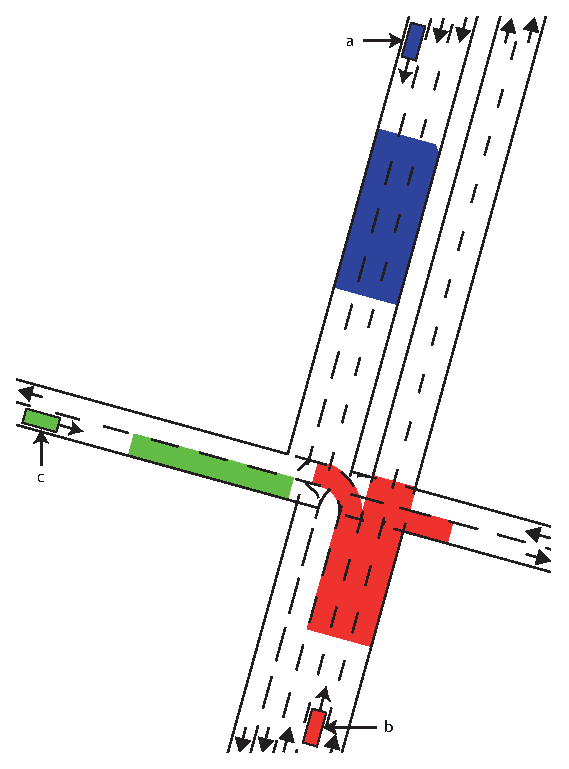
\includegraphics[height=0.5\textheight]{./figures/Scenario_Intersection_Occ_1,5-2,0s_final.eps}
	} \\
	\vspace{1em}
	Initial configuration and $\mathcal{O}(t)$ for $t \in [\unit[1.5]{s}, \unit[2.0]{s}]$
\end{center}

\end{frame}

\begin{frame}{Conclusions}

\begin{itemize}
\item Item
\vfill \item  Item
\vfill \item  Item
\end{itemize}

\end{frame}


begin{frame}
 \frametitle{Ballistic Integration Model }

   Distance and Velocity Equations:
   \begin{columns}[c]
       \begin{column}{0.5\hsize}\centering
       $$ \small s(k+1) = s(k) + dt \cdot v(k) + \frac{dt^2}{2} a(k) $$    
       \end{column}

       \begin{column}{0.5\hsize}
       $$ \small v(k+1) = v(k) + dt \cdot a(k) $$
       \end{column}
   \end{columns}

   \hfil

   \hfil

   \hfil

onslide<2>{

   Acceleration Equations:
   \begin{columns}[c]
       \begin{column}{0.5\hsize}
           \centering
           $$a(k) = \frac{2}{dt^2} \Bigl( s(k+1) - s(k) - dt \cdot v(k) \Bigr)$$
       \end{column}

       \begin{column}{0.5\hsize}
           \centering
           $$ a(k) = \frac{1}{dt} \Bigl( v(k+1) - v(k) \Bigr)$$
       \end{column}
   \end{columns}
}
end{frame}

\begin{frame}
  \frametitle{Results: Integration Method}
  \begin{figure}
    \centering
    \begin{minipage}[b]{0.45\linewidth}
      \centering
      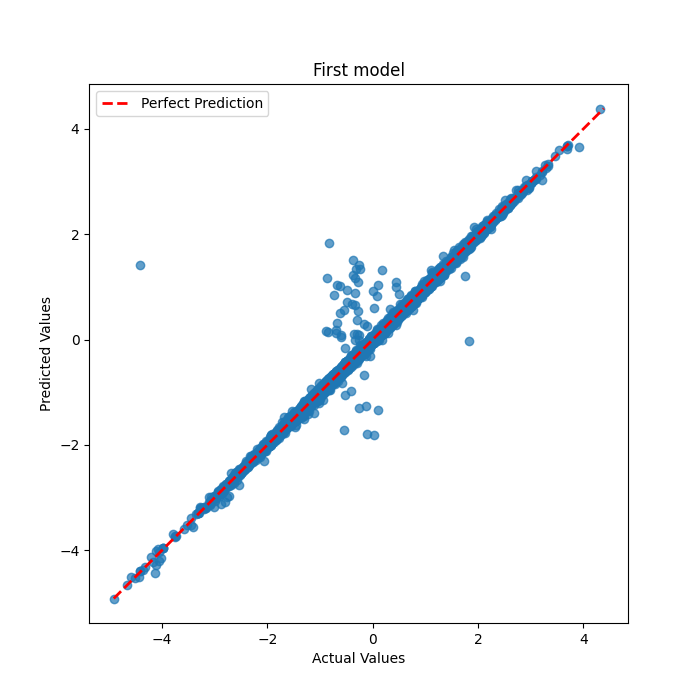
\includegraphics[width=\textwidth]{figures/graphs/First model.png}
    \end{minipage}
    \begin{minipage}[b]{0.45\linewidth}
      \centering
      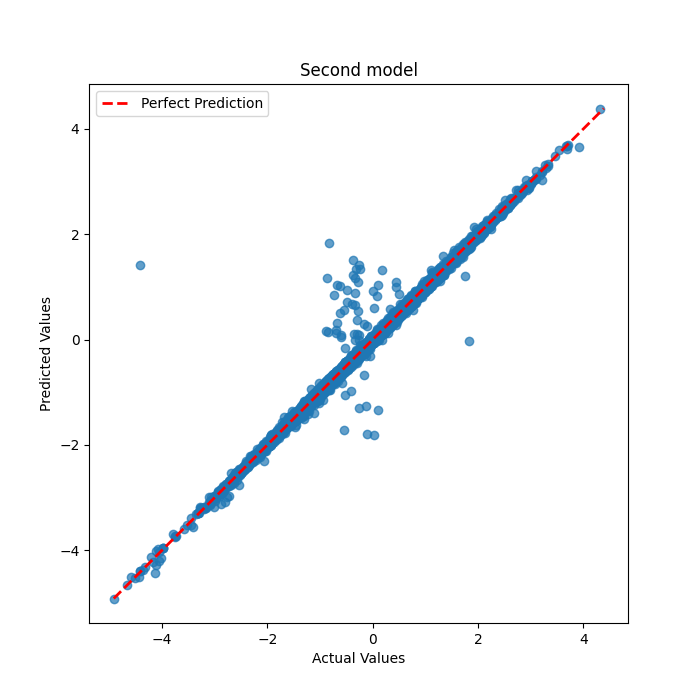
\includegraphics[width=\textwidth]{figures/graphs/Second model.png}
    \end{minipage}
  \end{figure}
\end{frame}

\begin{frame}
  \frametitle{Results: Integration Method}
    \center Video demo of predicted car
\end{frame}

\begin{frame}
  \frametitle{Our Integration Model }
    Our Distance and Velocity Equations:
\onslide<2, 3>{
    \begin{align*}
    s(t+1) &= s(t) + dt \cdot v(t)+ c_1 a(t) + c_2 a(t-1) \\
    v(t+1) &= v(t) + c_3 a(t) + c_4 a(t-1)
    \end{align*}

    \hfil
}
\onslide<3>{

    Our Acceleration Equations:
    \begin{align*}
    a(k) &= - \overline c_1 a(k-1)  + \overline c_2 \bigl( s(k+1) - s(k) - dt \cdot  v(k)\bigr)\\
    a(k) &= - \overline c_3 a(k-1)  + \overline c_4 \bigl( v(k+1) - v(k) \bigr) 
    \end{align*}
}

\end{frame}


\begin{frame}
  \frametitle{Our Integration Model}
  \onslide<1->{
    Model in matrix form:
    \begin{center}
      \scriptsize
      \begin{align*}
        \begin{bmatrix} a(k) \\ a(k) \end{bmatrix}
        &=
        \begin{bmatrix} 
            -a(k-1) & s(k+1) - s(k) - dt \cdot v(k) & 0 & 0   \\
            0 & 0 &-a(k-1) & v(k+1) - v(k) 
        \end{bmatrix}
        \begin{bmatrix}
            \overline{\textcolor{red}{c_1}} \\
            \overline{\textcolor{red}{c_2}} \\
            \overline{\textcolor{red}{c_3}} \\
            \overline{\textcolor{red}{c_4}} \\
        \end{bmatrix}
      \end{align*}
    \end{center}
  }
  \hfil

  \hfil

  \hfil

  \onslide<2->{
    $\Rightarrow$ This can be solved using linear regression.
  }
\end{frame}

\begin{frame}
  \frametitle{Results: Integration Method}
  \begin{figure}
    \centering
    \begin{minipage}[b]{0.45\linewidth}
        Accuracy of the prediction for the acceleration using the Ballistic Integration method (MSE):  4.3249e-02
    \end{minipage}
    \begin{minipage}[b]{0.45\linewidth}
      \centering
        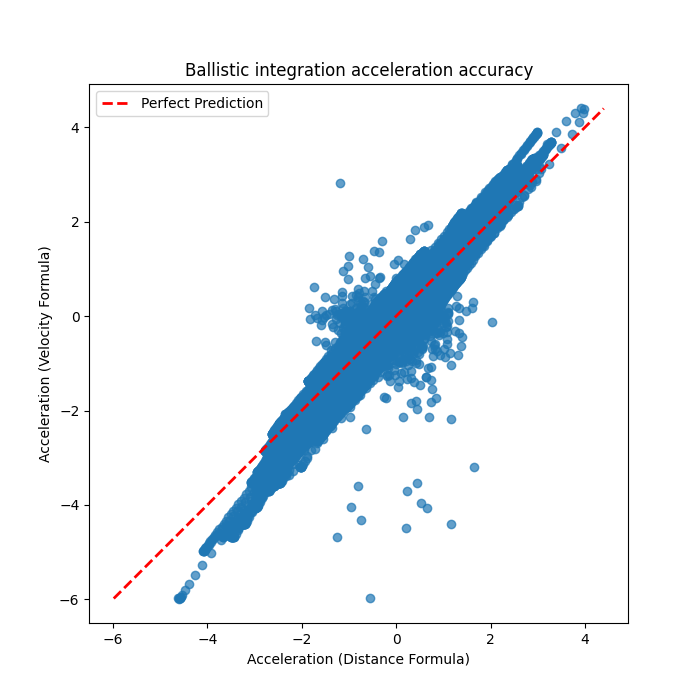
\includegraphics[width=\textwidth]{figures/graphs/Ballistic integration acceleration accuracy.png}
    \end{minipage}
  \end{figure}
\end{frame}


\begin{frame}
  \frametitle{Previous Integration Model - Accuracy}
  Accuracy of the prediction for the acceleration using the Ballistic Integration method (MSE):  4.3249e-02
  \begin{figure}
      \centering
        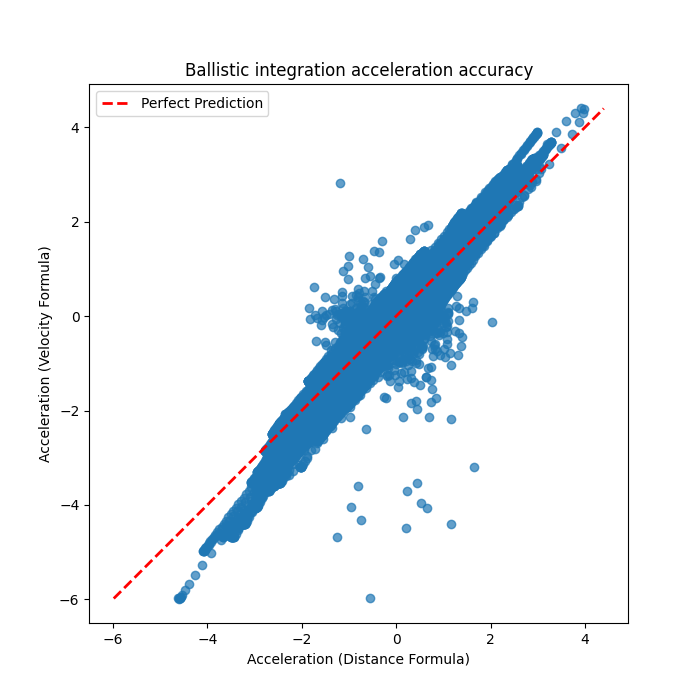
\includegraphics[width=0.5 \textwidth]{figures/graphs/Ballistic integration acceleration accuracy.png}
  \end{figure}

\end{frame}

\begin{frame}
  \frametitle{Results: Integration Method}
  Accuracy of the prediction for the acceleration (MSE): 3.0955e-03
  \begin{figure}
      \centering
        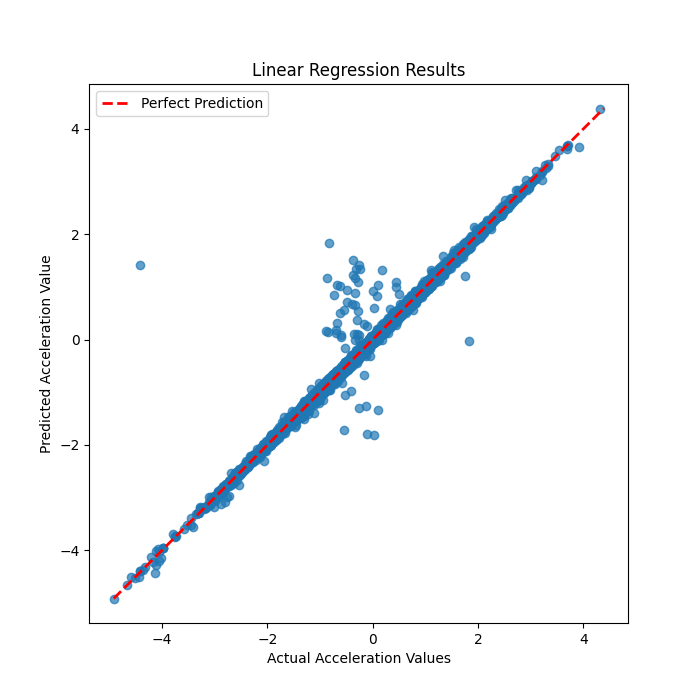
\includegraphics[width=0.6 \textwidth]{figures/graphs/Linear Regression Results.png}
  \end{figure}
\end{frame}



\begin{frame}
  \frametitle{Previous Integration Model }
    Distance and Velocity Equations (Ballistic Integration):
    \onslide<2, 3, 4>{
    \begin{align*}
        s(k+1) &= s(k) + dt \cdot v(k) + \frac{dt^2}{2} \color{blue}{a(k)} \\
        v(k+1) &= v(k) + dt \cdot                       \color{blue}{a(k)}
    \end{align*}

    }
    \onslide<3, 4>{

    \hfil

    Acceleration Equations (Rearranged):
    \begin{align*}
    \color{blue}{a(k)} &= \frac{2}{dt^2} \Bigl( s(k+1) - s(k) - dt \cdot v(k) \Bigr)\\
    \color{blue}{a(k)} &= \frac{1}{dt} \Bigl( v(k+1) - v(k) \Bigr)
    \end{align*}
    }
    \onslide<4>{

      \textbf{Problem:} Accelerations are not equal!
    }
\end{frame}



\begin{frame}
    \frametitle{Previous Integration Model - Accuracy}
    \begin{figure}
        \centering
        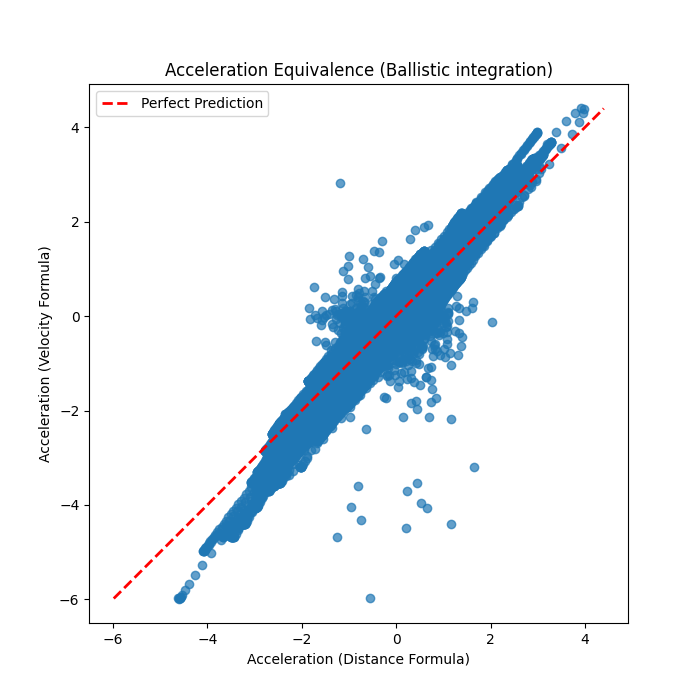
\includegraphics[width=0.65\textwidth]{figures/graphs/Acceleration Equivalence (Ballistic integration).png}
    \end{figure}
\end{frame}


\begin{frame}
  \frametitle{Our Integration Model - Matrix Form}
  \onslide<1->{
    Acceleration from Distance formula:
    \begin{align*}
        \begin{bmatrix} a(k) \\ \end{bmatrix}
        &=
        \begin{bmatrix}
            -a(k-1)  & v(k+1) - v(k)   \\ 
        \end{bmatrix}
        \begin{bmatrix}
            \overline{\textcolor{red}{c_1}} \\
            \overline{\textcolor{red}{c_2}} \\
        \end{bmatrix} \\
    \end{align*}

    Acceleration from Velocity formula:
    \begin{align*}
        \begin{bmatrix}
            a(k) \\ 
        \end{bmatrix}
        &=
        \begin{bmatrix}
            -a(k-1) &    s(k+1) - s(k) - dt \  v(k)   \\ 
        \end{bmatrix}
        \begin{bmatrix}
            \overline{\textcolor{red}{c_3}} \\
            \overline{\textcolor{red}{c_4}} \\
        \end{bmatrix}
    \end{align*}
  }

    \hfil

  \onslide<2->{
    $\Rightarrow$ This can be solved using linear regression.
  }

\end{frame}

\begin{frame}
    \textbf{Autonomous Driving Promise}
    \begin{itemize}[]
        \item Efficiency and Safety
    \end{itemize}

    \hfil

    \textbf{Challenges in Motion Prediction}
    \begin{itemize}[]
        \item Efficiency and Safety
    \end{itemize}

    \hfil

    \textbf{Multimodality}
    \begin{itemize}[]
        \item Scene Dependence
        \item Social Acceptability
    \end{itemize}

    \hfil

    \textbf{Crucial Understanding}
    \begin{itemize}[]
        \item Human-Driven Behavior Key
    \end{itemize}

    \hfil

    \textbf{Limitations of Current AI Tools}
    \begin{itemize}[]
        \item Control Perspective Absent
        \item Intent Interpretation Challenge
    \end{itemize}





\end{frame}




\begin{frame}

  \frametitle{Previous Integration Model }
    Distance and Velocity Equations (Ballistic Integration):
    \onslide<2, 3, 4>{
    \begin{align*}
        s(k+1) &= s(k) + dt \cdot v(k) + \frac{dt^2}{2} \color{blue}{a(k)} \\
        v(k+1) &= v(k) + dt \cdot                       \color{blue}{a(k)}
    \end{align*}

    }
    \onslide<3, 4>{

    \hfil

    Acceleration Equations (Rearranged):
    \begin{align*}
    \color{blue}{a(k)} &= \frac{2}{dt^2} \Bigl( s(k+1) - s(k) - dt \cdot v(k) \Bigr)\\
    \color{blue}{a(k)} &= \frac{1}{dt} \Bigl( v(k+1) - v(k) \Bigr)
    \end{align*}
    }
    \onslide<4>{

      \textbf{Problem:} Accelerations are not equal!
    }
\end{frame}

\begin{frame}
  \frametitle{Results: Integration Method}
  \begin{figure}
    \centering
    \begin{minipage}[b]{0.49\linewidth}

  \onslide<1, 2>{
        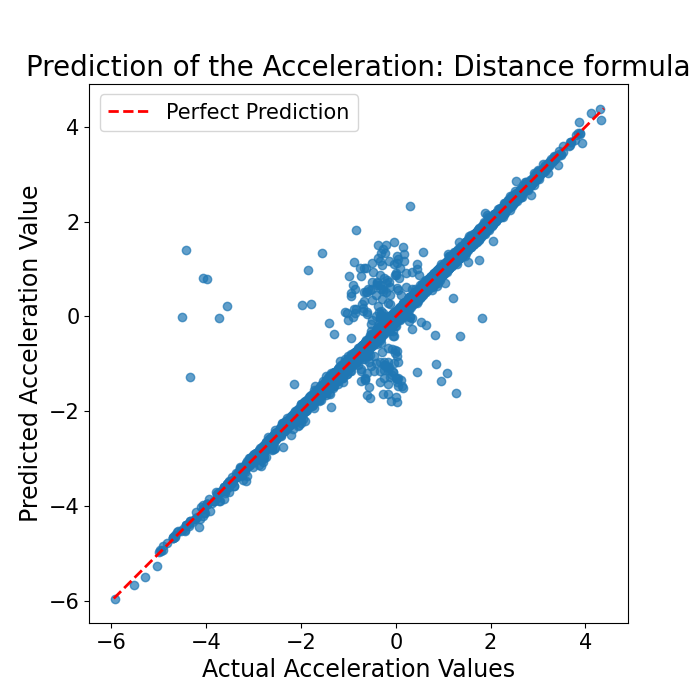
\includegraphics[width=\textwidth]{figures/graphs/Prediction of the Acceleration: Distance formula.png}
  }
    \end{minipage}
    \begin{minipage}[b]{0.49\linewidth}
      \centering
  \onslide<2>{
        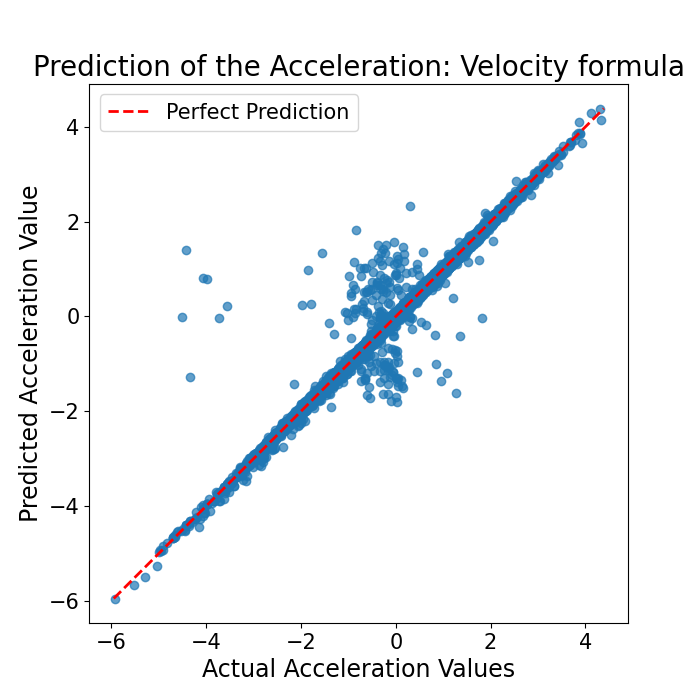
\includegraphics[width=\textwidth]{figures/graphs/Prediction of the Acceleration: Velocity formula.png}
  }
    \end{minipage}
  \end{figure}
\end{frame}


\begin{frame}
  \frametitle{Results}
    Summary:
    \begin{itemize}[<+->]
      \item Successfully implemented the filtering mechanism
      \item Able to filter out X different scenarios in Y datasets
      \item Found a better integration method where the accelerations match
      \item Able to visualize the integration method and modulate the movement of a car
    \end{itemize}
\end{frame}


\begin{frame}
  \frametitle{Previous Integration Model }
    Distance and Velocity Equations (Ballistic Integration):
    \onslide<2, 3, 4>{
    \begin{align*}
        s(k+1) &= s(k) + dt \cdot v(k) + \frac{dt^2}{2} \color{blue}{a(k)} \\
        v(k+1) &= v(k) + dt \cdot                       \color{blue}{a(k)}
    \end{align*}

    }
    \onslide<3, 4>{

    \hfil

    Acceleration Equations (Rearranged):
    \begin{align*}
    \color{blue}{a(k)} &= \frac{2}{dt^2} \Bigl( s(k+1) - s(k) - dt \cdot v(k) \Bigr)\\
    \color{blue}{a(k)} &= \frac{1}{dt} \Bigl( v(k+1) - v(k) \Bigr)
    \end{align*}
    }
    \onslide<4>{

      \textbf{Problem:} Accelerations are not equal!
    }
\end{frame}




\begin{frame}
  \begin{center}
  Thank you for your attention:)
  \end{center}
\end{frame}


\end{document}